\documentclass[twoside]{book}

% Packages required by doxygen
\usepackage{fixltx2e}
\usepackage{calc}
\usepackage{doxygen}
\usepackage[export]{adjustbox} % also loads graphicx
\usepackage{graphicx}
\usepackage[utf8]{inputenc}
\usepackage{makeidx}
\usepackage{multicol}
\usepackage{multirow}
\PassOptionsToPackage{warn}{textcomp}
\usepackage{textcomp}
\usepackage[nointegrals]{wasysym}
\usepackage[table]{xcolor}

% Font selection
\usepackage[T1]{fontenc}
\usepackage[scaled=.90]{helvet}
\usepackage{courier}
\usepackage{amssymb}
\usepackage{sectsty}
\renewcommand{\familydefault}{\sfdefault}
\allsectionsfont{%
  \fontseries{bc}\selectfont%
  \color{darkgray}%
}
\renewcommand{\DoxyLabelFont}{%
  \fontseries{bc}\selectfont%
  \color{darkgray}%
}
\newcommand{\+}{\discretionary{\mbox{\scriptsize$\hookleftarrow$}}{}{}}

% Page & text layout
\usepackage{geometry}
\geometry{%
  a4paper,%
  top=2.5cm,%
  bottom=2.5cm,%
  left=2.5cm,%
  right=2.5cm%
}
\tolerance=750
\hfuzz=15pt
\hbadness=750
\setlength{\emergencystretch}{15pt}
\setlength{\parindent}{0cm}
\setlength{\parskip}{3ex plus 2ex minus 2ex}
\makeatletter
\renewcommand{\paragraph}{%
  \@startsection{paragraph}{4}{0ex}{-1.0ex}{1.0ex}{%
    \normalfont\normalsize\bfseries\SS@parafont%
  }%
}
\renewcommand{\subparagraph}{%
  \@startsection{subparagraph}{5}{0ex}{-1.0ex}{1.0ex}{%
    \normalfont\normalsize\bfseries\SS@subparafont%
  }%
}
\makeatother

% Headers & footers
\usepackage{fancyhdr}
\pagestyle{fancyplain}
\fancyhead[LE]{\fancyplain{}{\bfseries\thepage}}
\fancyhead[CE]{\fancyplain{}{}}
\fancyhead[RE]{\fancyplain{}{\bfseries\leftmark}}
\fancyhead[LO]{\fancyplain{}{\bfseries\rightmark}}
\fancyhead[CO]{\fancyplain{}{}}
\fancyhead[RO]{\fancyplain{}{\bfseries\thepage}}
\fancyfoot[LE]{\fancyplain{}{}}
\fancyfoot[CE]{\fancyplain{}{}}
\fancyfoot[RE]{\fancyplain{}{\bfseries\scriptsize Generated by Doxygen }}
\fancyfoot[LO]{\fancyplain{}{\bfseries\scriptsize Generated by Doxygen }}
\fancyfoot[CO]{\fancyplain{}{}}
\fancyfoot[RO]{\fancyplain{}{}}
\renewcommand{\footrulewidth}{0.4pt}
\renewcommand{\chaptermark}[1]{%
  \markboth{#1}{}%
}
\renewcommand{\sectionmark}[1]{%
  \markright{\thesection\ #1}%
}

% Indices & bibliography
\usepackage{natbib}
\usepackage[titles]{tocloft}
\setcounter{tocdepth}{3}
\setcounter{secnumdepth}{5}
\makeindex

% Hyperlinks (required, but should be loaded last)
\usepackage{ifpdf}
\ifpdf
  \usepackage[pdftex,pagebackref=true]{hyperref}
\else
  \usepackage[ps2pdf,pagebackref=true]{hyperref}
\fi
\hypersetup{%
  colorlinks=true,%
  linkcolor=blue,%
  citecolor=blue,%
  unicode%
}

% Custom commands
\newcommand{\clearemptydoublepage}{%
  \newpage{\pagestyle{empty}\cleardoublepage}%
}

\usepackage{caption}
\captionsetup{labelsep=space,justification=centering,font={bf},singlelinecheck=off,skip=4pt,position=top}

%===== C O N T E N T S =====

\begin{document}

% Titlepage & ToC
\hypersetup{pageanchor=false,
             bookmarksnumbered=true,
             pdfencoding=unicode
            }
\pagenumbering{alph}
\begin{titlepage}
\vspace*{7cm}
\begin{center}%
{\Large Szachy \\[1ex]\large 1.\+0 }\\
\vspace*{1cm}
{\large Generated by Doxygen 1.8.13}\\
\end{center}
\end{titlepage}
\clearemptydoublepage
\pagenumbering{roman}
\tableofcontents
\clearemptydoublepage
\pagenumbering{arabic}
\hypersetup{pageanchor=true}

%--- Begin generated contents ---
\chapter{chess\+Test2}
\label{md__r_e_a_d_m_e}
\Hypertarget{md__r_e_a_d_m_e}
Projekt na J\+PO 
\chapter{Hierarchical Index}
\section{Class Hierarchy}
This inheritance list is sorted roughly, but not completely, alphabetically\+:\begin{DoxyCompactList}
\item \contentsline{section}{chess\+Piece}{\pageref{classchess_piece}}{}
\item Q\+Dialog\begin{DoxyCompactList}
\item \contentsline{section}{chess\+Settings}{\pageref{classchess_settings}}{}
\end{DoxyCompactList}
\item Q\+Label\begin{DoxyCompactList}
\item \contentsline{section}{chess\+Square}{\pageref{classchess_square}}{}
\end{DoxyCompactList}
\item Q\+Main\+Window\begin{DoxyCompactList}
\item \contentsline{section}{chess\+Game}{\pageref{classchess_game}}{}
\end{DoxyCompactList}
\item Q\+Widget\begin{DoxyCompactList}
\item \contentsline{section}{chess\+Board}{\pageref{classchess_board}}{}
\item \contentsline{section}{chess\+Panel}{\pageref{classchess_panel}}{}
\end{DoxyCompactList}
\end{DoxyCompactList}

\chapter{Class Index}
\section{Class List}
Here are the classes, structs, unions and interfaces with brief descriptions\+:\begin{DoxyCompactList}
\item\contentsline{section}{\hyperlink{classchess_board}{chess\+Board} \\*Klasa \hyperlink{classchess_board}{chess\+Board} odpowiada za prawidłowe wyświetlanie i działanie szachownicy }{\pageref{classchess_board}}{}
\item\contentsline{section}{\hyperlink{classchess_game}{chess\+Game} \\*Główna klasa gry. Odpowiada za poprawne działania i wyświetlanie okna }{\pageref{classchess_game}}{}
\item\contentsline{section}{\hyperlink{classchess_panel}{chess\+Panel} \\*Odpowiada za prawidłowe wyświetlanie i działanie panelu bocznego }{\pageref{classchess_panel}}{}
\item\contentsline{section}{\hyperlink{classchess_piece}{chess\+Piece} \\*Klasa reprezentująca pojedynczą figurę }{\pageref{classchess_piece}}{}
\item\contentsline{section}{\hyperlink{classchess_settings}{chess\+Settings} \\*Odpowiada za prawidłowe wyświetlanie i działanie okna ustawień }{\pageref{classchess_settings}}{}
\item\contentsline{section}{\hyperlink{classchess_square}{chess\+Square} \\*Klasa reprezentująca pojedyncze pole na szachownicy }{\pageref{classchess_square}}{}
\end{DoxyCompactList}

\chapter{Class Documentation}
\hypertarget{classchess_board}{}\section{chess\+Board Class Reference}
\label{classchess_board}\index{chess\+Board@{chess\+Board}}


Klasa \hyperlink{classchess_board}{chess\+Board} odpowiada za prawidłowe wyświetlanie i działanie szachownicy.  


Inheritance diagram for chess\+Board\+:\begin{figure}[H]
\begin{center}
\leavevmode
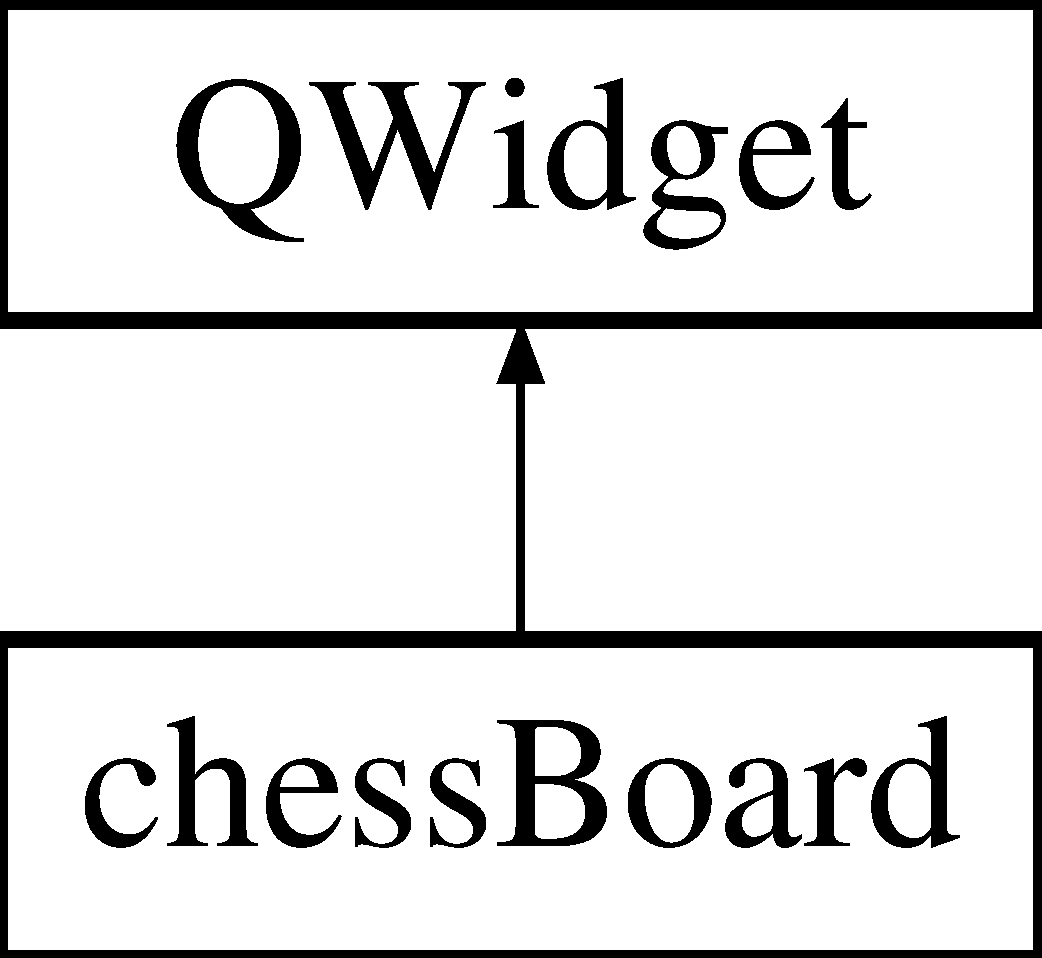
\includegraphics[height=2.000000cm]{classchess_board}
\end{center}
\end{figure}
\subsection*{Public Slots}
\begin{DoxyCompactItemize}
\item 
void \hyperlink{classchess_board_aa867893a425aa624b21e9c8185198d3e}{validate\+Click} (int x, int y)
\begin{DoxyCompactList}\small\item\em Funkcja analizująca kliknięte pole. \end{DoxyCompactList}\end{DoxyCompactItemize}
\subsection*{Signals}
\begin{DoxyCompactItemize}
\item 
\mbox{\Hypertarget{classchess_board_acc9cef750420c74bfc72b07a94799c7b}\label{classchess_board_acc9cef750420c74bfc72b07a94799c7b}} 
void \hyperlink{classchess_board_acc9cef750420c74bfc72b07a94799c7b}{check\+Mate} (int player)
\begin{DoxyCompactList}\small\item\em Sygnał \char`\"{}\+Szach mat\char`\"{} -\/ wysyłany po zbiciu króla. \end{DoxyCompactList}\item 
\mbox{\Hypertarget{classchess_board_a20775bae5ea49615cf79615d01f9f469}\label{classchess_board_a20775bae5ea49615cf79615d01f9f469}} 
void \hyperlink{classchess_board_a20775bae5ea49615cf79615d01f9f469}{next\+Move} ()
\begin{DoxyCompactList}\small\item\em Sygnał wysyłany każdorazowo po wykonaniu ruchu. \end{DoxyCompactList}\item 
\mbox{\Hypertarget{classchess_board_ab353f1caafb54b0efa14621a38687711}\label{classchess_board_ab353f1caafb54b0efa14621a38687711}} 
void \hyperlink{classchess_board_ab353f1caafb54b0efa14621a38687711}{new\+Lost} ()
\begin{DoxyCompactList}\small\item\em Sygnał wysyłany każdorazowo po zbiciu figury. \end{DoxyCompactList}\end{DoxyCompactItemize}
\subsection*{Public Member Functions}
\begin{DoxyCompactItemize}
\item 
\hyperlink{classchess_board_a3ffc09a4d95deaca0f6744ae25bb4f62}{chess\+Board} (Q\+Widget $\ast$parent=0)
\begin{DoxyCompactList}\small\item\em Konstruktor klasy \hyperlink{classchess_board}{chess\+Board}. \end{DoxyCompactList}\item 
void \hyperlink{classchess_board_a429d72a00c66352a9657cba0625c981b}{generate\+Chess\+Pieces} ()
\begin{DoxyCompactList}\small\item\em Generuje figury na szachownicy. \end{DoxyCompactList}\item 
void \hyperlink{classchess_board_abc343d0274a5d10c01934d3b1da56c1f}{update\+Colors} (Q\+String newblack, Q\+String newwhite, Q\+String newselect, Q\+String newattack)
\begin{DoxyCompactList}\small\item\em Ustawia nowy zestaw kolorów na szachownicy. \end{DoxyCompactList}\item 
void \hyperlink{classchess_board_ab8a0e470df04224d40a38f99fe4232bc}{reset\+Chessboard} ()
\begin{DoxyCompactList}\small\item\em Czyści szachownicę -\/ usuwa wszystkie pionki (również z listy), resetuje numer gracza. \end{DoxyCompactList}\item 
void \hyperlink{classchess_board_a3d7939233de9607a91357c3616f5db67}{block\+All\+Squares} ()
\begin{DoxyCompactList}\small\item\em Funkcja ustawia wszystkie pola na nieaktywne. \end{DoxyCompactList}\item 
void \hyperlink{classchess_board_a43133dc6f58be4b00cc54a7ba744f69a}{read\+From\+Text} (Q\+String line)
\begin{DoxyCompactList}\small\item\em Funkcja wczytująca ruchy z tekstu (zapisane w notacji szachowaj) \end{DoxyCompactList}\item 
\hyperlink{classchess_board_a91541e52c3b570ad4e06914786f33002}{$\sim$chess\+Board} ()
\end{DoxyCompactItemize}
\subsection*{Public Attributes}
\begin{DoxyCompactItemize}
\item 
\mbox{\Hypertarget{classchess_board_a4a0184eb6e20074eec3fce6a08e0ff62}\label{classchess_board_a4a0184eb6e20074eec3fce6a08e0ff62}} 
Q\+String\+List \hyperlink{classchess_board_a4a0184eb6e20074eec3fce6a08e0ff62}{history}
\begin{DoxyCompactList}\small\item\em Lista stringów przechowująca historię ruchów w notacji szachowej. \end{DoxyCompactList}\end{DoxyCompactItemize}
\subsection*{Friends}
\begin{DoxyCompactItemize}
\item 
\mbox{\Hypertarget{classchess_board_a789fcbbf0675ebb167838f8f7e11fafa}\label{classchess_board_a789fcbbf0675ebb167838f8f7e11fafa}} 
class {\bfseries chess\+Settings}
\item 
\mbox{\Hypertarget{classchess_board_a9b25e97c3caab58490ce854e1e72e975}\label{classchess_board_a9b25e97c3caab58490ce854e1e72e975}} 
class {\bfseries chess\+Panel}
\end{DoxyCompactItemize}


\subsection{Detailed Description}
Klasa \hyperlink{classchess_board}{chess\+Board} odpowiada za prawidłowe wyświetlanie i działanie szachownicy. 

Klasa ta dziedziczy po Q\+Widget i wyświetla pustą szachownicę o standardowych kolorach szary-\/biały. 

\subsection{Constructor \& Destructor Documentation}
\mbox{\Hypertarget{classchess_board_a3ffc09a4d95deaca0f6744ae25bb4f62}\label{classchess_board_a3ffc09a4d95deaca0f6744ae25bb4f62}} 
\index{chess\+Board@{chess\+Board}!chess\+Board@{chess\+Board}}
\index{chess\+Board@{chess\+Board}!chess\+Board@{chess\+Board}}
\subsubsection{\texorpdfstring{chess\+Board()}{chessBoard()}}
{\footnotesize\ttfamily chess\+Board\+::chess\+Board (\begin{DoxyParamCaption}\item[{Q\+Widget $\ast$}]{parent = {\ttfamily 0} }\end{DoxyParamCaption})}



Konstruktor klasy \hyperlink{classchess_board}{chess\+Board}. 

Konstruktor klasy \hyperlink{classchess_board}{chess\+Board} tworzy pustą szachownicę składającą sie z obiektów typu \hyperlink{classchess_square}{chess\+Square} oraz ustawia domyślne kolory. \mbox{\Hypertarget{classchess_board_a91541e52c3b570ad4e06914786f33002}\label{classchess_board_a91541e52c3b570ad4e06914786f33002}} 
\index{chess\+Board@{chess\+Board}!````~chess\+Board@{$\sim$chess\+Board}}
\index{````~chess\+Board@{$\sim$chess\+Board}!chess\+Board@{chess\+Board}}
\subsubsection{\texorpdfstring{$\sim$chess\+Board()}{~chessBoard()}}
{\footnotesize\ttfamily chess\+Board\+::$\sim$chess\+Board (\begin{DoxyParamCaption}{ }\end{DoxyParamCaption})}


\begin{DoxyParams}{Parameters}
{\em x} & Współrzędna x kliknietego pola \\
\hline
{\em y} & Współrzędna x kliknietego pola\\
\hline
\end{DoxyParams}
Destruktor usuwa wszystkie pola z szachownicy. 

\subsection{Member Function Documentation}
\mbox{\Hypertarget{classchess_board_a3d7939233de9607a91357c3616f5db67}\label{classchess_board_a3d7939233de9607a91357c3616f5db67}} 
\index{chess\+Board@{chess\+Board}!block\+All\+Squares@{block\+All\+Squares}}
\index{block\+All\+Squares@{block\+All\+Squares}!chess\+Board@{chess\+Board}}
\subsubsection{\texorpdfstring{block\+All\+Squares()}{blockAllSquares()}}
{\footnotesize\ttfamily void chess\+Board\+::block\+All\+Squares (\begin{DoxyParamCaption}{ }\end{DoxyParamCaption})}



Funkcja ustawia wszystkie pola na nieaktywne. 

Ustawia wszystkie pola jako nieaktywne. Funkcja wywoływana po zakończeniu gry. \mbox{\Hypertarget{classchess_board_a429d72a00c66352a9657cba0625c981b}\label{classchess_board_a429d72a00c66352a9657cba0625c981b}} 
\index{chess\+Board@{chess\+Board}!generate\+Chess\+Pieces@{generate\+Chess\+Pieces}}
\index{generate\+Chess\+Pieces@{generate\+Chess\+Pieces}!chess\+Board@{chess\+Board}}
\subsubsection{\texorpdfstring{generate\+Chess\+Pieces()}{generateChessPieces()}}
{\footnotesize\ttfamily void chess\+Board\+::generate\+Chess\+Pieces (\begin{DoxyParamCaption}{ }\end{DoxyParamCaption})}



Generuje figury na szachownicy. 

Generuje nowy zestaw figur i przypisuje je do szachownicy na domyślnych pozycjach. \mbox{\Hypertarget{classchess_board_a43133dc6f58be4b00cc54a7ba744f69a}\label{classchess_board_a43133dc6f58be4b00cc54a7ba744f69a}} 
\index{chess\+Board@{chess\+Board}!read\+From\+Text@{read\+From\+Text}}
\index{read\+From\+Text@{read\+From\+Text}!chess\+Board@{chess\+Board}}
\subsubsection{\texorpdfstring{read\+From\+Text()}{readFromText()}}
{\footnotesize\ttfamily void chess\+Board\+::read\+From\+Text (\begin{DoxyParamCaption}\item[{Q\+String}]{line }\end{DoxyParamCaption})}



Funkcja wczytująca ruchy z tekstu (zapisane w notacji szachowaj) 


\begin{DoxyParams}{Parameters}
{\em line} & Pojedyncza linia z pliku tekstowego. Np\+: \char`\"{}\+A2 B2\char`\"{}\\
\hline
\end{DoxyParams}
Funkcja analizuje współrzędne pola na szachownicy (x, y). Wywoływana jest przez sygnał clicked() z klasy \hyperlink{classchess_square}{chess\+Square}. W przypadku gdy na danym polu znajduje się figura, funkcja rozpoznaje typ figury, a następnie aktywuje te pola na które dana figura może się przemieścić. W przypadku gdy na danym polu nie ma żadnej figury, wywoływana jest funkcja move(). \mbox{\Hypertarget{classchess_board_ab8a0e470df04224d40a38f99fe4232bc}\label{classchess_board_ab8a0e470df04224d40a38f99fe4232bc}} 
\index{chess\+Board@{chess\+Board}!reset\+Chessboard@{reset\+Chessboard}}
\index{reset\+Chessboard@{reset\+Chessboard}!chess\+Board@{chess\+Board}}
\subsubsection{\texorpdfstring{reset\+Chessboard()}{resetChessboard()}}
{\footnotesize\ttfamily void chess\+Board\+::reset\+Chessboard (\begin{DoxyParamCaption}{ }\end{DoxyParamCaption})}



Czyści szachownicę -\/ usuwa wszystkie pionki (również z listy), resetuje numer gracza. 

Usuwa ona wszystkie pionki (również z listy straconych figur). Ponadto resetuje ona numer gracza. \mbox{\Hypertarget{classchess_board_abc343d0274a5d10c01934d3b1da56c1f}\label{classchess_board_abc343d0274a5d10c01934d3b1da56c1f}} 
\index{chess\+Board@{chess\+Board}!update\+Colors@{update\+Colors}}
\index{update\+Colors@{update\+Colors}!chess\+Board@{chess\+Board}}
\subsubsection{\texorpdfstring{update\+Colors()}{updateColors()}}
{\footnotesize\ttfamily void chess\+Board\+::update\+Colors (\begin{DoxyParamCaption}\item[{Q\+String}]{newblack,  }\item[{Q\+String}]{newwhite,  }\item[{Q\+String}]{newselect,  }\item[{Q\+String}]{newattack }\end{DoxyParamCaption})}



Ustawia nowy zestaw kolorów na szachownicy. 


\begin{DoxyParams}{Parameters}
{\em newblack} & Nowy kolor pola czarnego \\
\hline
{\em newwhite} & Nowy kolor pola białego \\
\hline
{\em newselect} & Nowy kolor pola zaznaczonego \\
\hline
{\em newattack} & Nowy kolor pola atakującego\\
\hline
\end{DoxyParams}
Ustawia nowy zestaw kolorów na szachownicy. W jej argumentach podawane są ustawiane kolory w postaci tekstowej (Q\+String). \mbox{\Hypertarget{classchess_board_aa867893a425aa624b21e9c8185198d3e}\label{classchess_board_aa867893a425aa624b21e9c8185198d3e}} 
\index{chess\+Board@{chess\+Board}!validate\+Click@{validate\+Click}}
\index{validate\+Click@{validate\+Click}!chess\+Board@{chess\+Board}}
\subsubsection{\texorpdfstring{validate\+Click}{validateClick}}
{\footnotesize\ttfamily void chess\+Board\+::validate\+Click (\begin{DoxyParamCaption}\item[{int}]{x,  }\item[{int}]{y }\end{DoxyParamCaption})\hspace{0.3cm}{\ttfamily [slot]}}



Funkcja analizująca kliknięte pole. 


\begin{DoxyParams}{Parameters}
{\em x} & Współrzędna x kliknietego pola \\
\hline
{\em y} & Współrzędna x kliknietego pola\\
\hline
\end{DoxyParams}
Funkcja analizuje współrzędne pola na szachownicy (x, y). Wywoływana jest przez sygnał clicked() z klasy \hyperlink{classchess_square}{chess\+Square}. W przypadku gdy na danym polu znajduje się figura, funkcja rozpoznaje typ figury, a następnie aktywuje te pola na które dana figura może się przemieścić. W przypadku gdy na danym polu nie ma żadnej figury, wywoływana jest funkcja move(). 

The documentation for this class was generated from the following files\+:\begin{DoxyCompactItemize}
\item 
chessboard.\+h\item 
chessboard.\+cpp\end{DoxyCompactItemize}

\hypertarget{classchess_game}{}\section{chess\+Game Class Reference}
\label{classchess_game}\index{chess\+Game@{chess\+Game}}


Główna klasa gry. Odpowiada za poprawne działania i wyświetlanie okna.  


Inheritance diagram for chess\+Game\+:\begin{figure}[H]
\begin{center}
\leavevmode
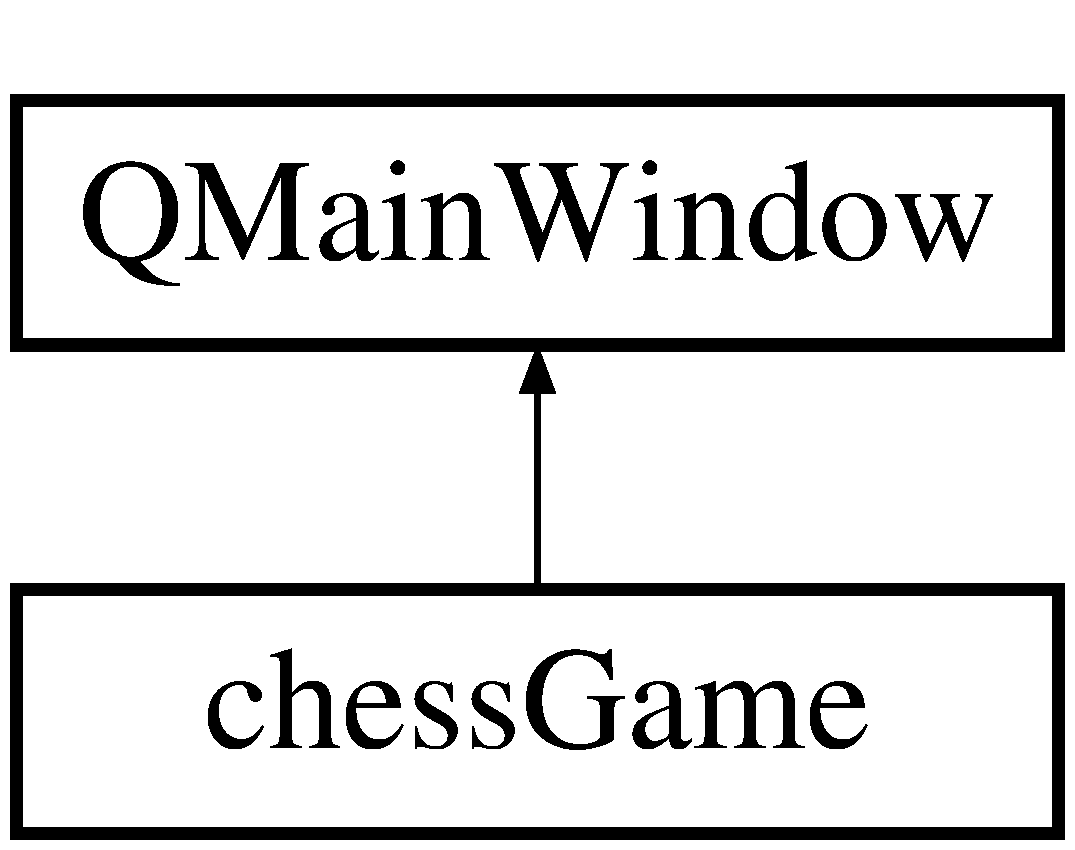
\includegraphics[height=2.000000cm]{classchess_game}
\end{center}
\end{figure}
\subsection*{Public Slots}
\begin{DoxyCompactItemize}
\item 
\mbox{\Hypertarget{classchess_game_a230eb38f254315b36cd363d9934d4945}\label{classchess_game_a230eb38f254315b36cd363d9934d4945}} 
void \hyperlink{classchess_game_a230eb38f254315b36cd363d9934d4945}{new\+\_\+game} ()
\begin{DoxyCompactList}\small\item\em Tworzy nową sesję gry. \end{DoxyCompactList}\item 
\mbox{\Hypertarget{classchess_game_a5aa2f3514c1ef832a80ab5a10288c20e}\label{classchess_game_a5aa2f3514c1ef832a80ab5a10288c20e}} 
void \hyperlink{classchess_game_a5aa2f3514c1ef832a80ab5a10288c20e}{save\+\_\+game} ()
\begin{DoxyCompactList}\small\item\em Zapisuje obecny stan gry do pliku. \end{DoxyCompactList}\item 
\mbox{\Hypertarget{classchess_game_aff9965791d6a11efb08d6c483db6371b}\label{classchess_game_aff9965791d6a11efb08d6c483db6371b}} 
void \hyperlink{classchess_game_aff9965791d6a11efb08d6c483db6371b}{save\+As\+\_\+game} ()
\begin{DoxyCompactList}\small\item\em Zapisuje obecny stan gry do nowego pliku. \end{DoxyCompactList}\item 
\mbox{\Hypertarget{classchess_game_a5e8b9a01b5d091579e7f13fe742c85b1}\label{classchess_game_a5e8b9a01b5d091579e7f13fe742c85b1}} 
void \hyperlink{classchess_game_a5e8b9a01b5d091579e7f13fe742c85b1}{open\+\_\+game} ()
\begin{DoxyCompactList}\small\item\em Otwiera i odczytuje stan gry z pliku. \end{DoxyCompactList}\item 
\mbox{\Hypertarget{classchess_game_a0fec48a8caa52eca9bb109b1ab7d5aa9}\label{classchess_game_a0fec48a8caa52eca9bb109b1ab7d5aa9}} 
void \hyperlink{classchess_game_a0fec48a8caa52eca9bb109b1ab7d5aa9}{close\+\_\+window} ()
\begin{DoxyCompactList}\small\item\em Zamyka grę \end{DoxyCompactList}\item 
\mbox{\Hypertarget{classchess_game_af4636d3a148b8e910ac093bf419fbac7}\label{classchess_game_af4636d3a148b8e910ac093bf419fbac7}} 
void \hyperlink{classchess_game_af4636d3a148b8e910ac093bf419fbac7}{open\+\_\+settings} ()
\begin{DoxyCompactList}\small\item\em Otwiera okno ustawień \end{DoxyCompactList}\item 
\mbox{\Hypertarget{classchess_game_a00156441ff76452fd40b572683ea99b9}\label{classchess_game_a00156441ff76452fd40b572683ea99b9}} 
void \hyperlink{classchess_game_a00156441ff76452fd40b572683ea99b9}{about\+\_\+qt} ()
\begin{DoxyCompactList}\small\item\em Otwiera okno \char`\"{}\+About Qt\char`\"{}. \end{DoxyCompactList}\item 
\mbox{\Hypertarget{classchess_game_a86245fb64348f772be40001d4f063f03}\label{classchess_game_a86245fb64348f772be40001d4f063f03}} 
void \hyperlink{classchess_game_a86245fb64348f772be40001d4f063f03}{about\+\_\+game} ()
\begin{DoxyCompactList}\small\item\em Otwiera okno \char`\"{}\+O grze\char`\"{}. \end{DoxyCompactList}\item 
\mbox{\Hypertarget{classchess_game_a209b5541bf8d34b7f9ff0c48972bf972}\label{classchess_game_a209b5541bf8d34b7f9ff0c48972bf972}} 
void \hyperlink{classchess_game_a209b5541bf8d34b7f9ff0c48972bf972}{game\+\_\+over} (int player)
\begin{DoxyCompactList}\small\item\em Kończy aktualną grę i wyświetla komunikat o zwycięstwie. \end{DoxyCompactList}\item 
\mbox{\Hypertarget{classchess_game_aa53efb2e6476d9a7445e7a166ebe023b}\label{classchess_game_aa53efb2e6476d9a7445e7a166ebe023b}} 
void \hyperlink{classchess_game_aa53efb2e6476d9a7445e7a166ebe023b}{set\+Not\+Saved} ()
\begin{DoxyCompactList}\small\item\em Ustawia stan gry na niezapisany. \end{DoxyCompactList}\end{DoxyCompactItemize}
\subsection*{Public Member Functions}
\begin{DoxyCompactItemize}
\item 
\mbox{\Hypertarget{classchess_game_a9d6406de47a97ca52a4016a5caf9f598}\label{classchess_game_a9d6406de47a97ca52a4016a5caf9f598}} 
{\bfseries chess\+Game} (Q\+Widget $\ast$parent=0)
\end{DoxyCompactItemize}
\subsection*{Protected Member Functions}
\begin{DoxyCompactItemize}
\item 
\mbox{\Hypertarget{classchess_game_aa030ac566950d641e55f7d5b9d249f7c}\label{classchess_game_aa030ac566950d641e55f7d5b9d249f7c}} 
void {\bfseries close\+Event} (Q\+Close\+Event $\ast$event)
\end{DoxyCompactItemize}


\subsection{Detailed Description}
Główna klasa gry. Odpowiada za poprawne działania i wyświetlanie okna. 

Klasa ta dziedziczy po Q\+Main\+Window. Tworzy nowe okno, a w nim szachownicę oraz panel. Odpowiada za prawidłowe działanie pasków i przycisków. 

The documentation for this class was generated from the following files\+:\begin{DoxyCompactItemize}
\item 
chessgame.\+h\item 
chessgame.\+cpp\end{DoxyCompactItemize}

\hypertarget{classchess_panel}{}\section{chess\+Panel Class Reference}
\label{classchess_panel}\index{chess\+Panel@{chess\+Panel}}


Odpowiada za prawidłowe wyświetlanie i działanie panelu bocznego.  


Inheritance diagram for chess\+Panel\+:\begin{figure}[H]
\begin{center}
\leavevmode
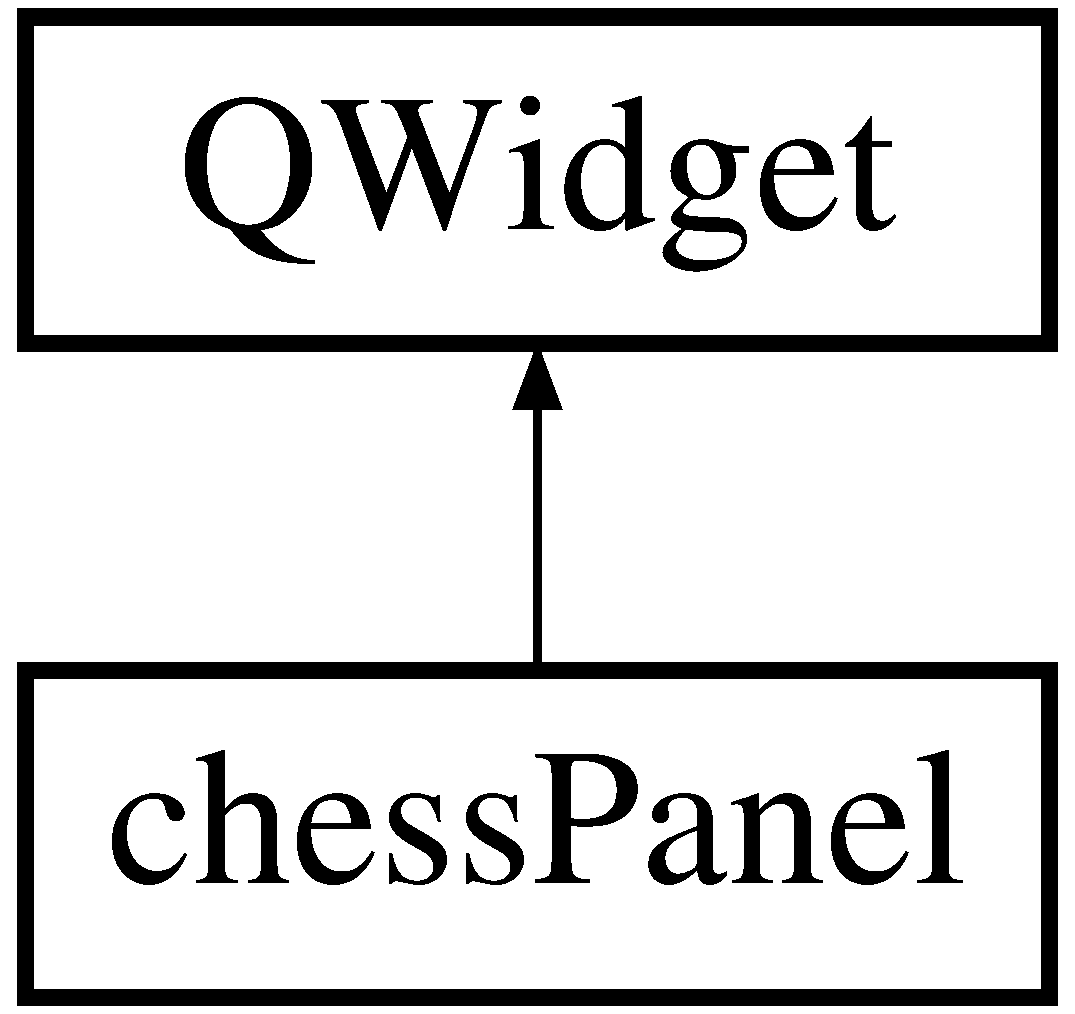
\includegraphics[height=2.000000cm]{classchess_panel}
\end{center}
\end{figure}
\subsection*{Public Slots}
\begin{DoxyCompactItemize}
\item 
\mbox{\Hypertarget{classchess_panel_adeab3d504a94b4380487c3a04a10441e}\label{classchess_panel_adeab3d504a94b4380487c3a04a10441e}} 
void \hyperlink{classchess_panel_adeab3d504a94b4380487c3a04a10441e}{update\+Lost} ()
\begin{DoxyCompactList}\small\item\em Aktualizuje listę ze straconymi pionkami. \end{DoxyCompactList}\item 
\mbox{\Hypertarget{classchess_panel_a65f79990c4a6fdd8b26c469d605d44e8}\label{classchess_panel_a65f79990c4a6fdd8b26c469d605d44e8}} 
void \hyperlink{classchess_panel_a65f79990c4a6fdd8b26c469d605d44e8}{update\+Current\+Player} ()
\begin{DoxyCompactList}\small\item\em Zmienia aktualny numer gracza. \end{DoxyCompactList}\end{DoxyCompactItemize}
\subsection*{Public Member Functions}
\begin{DoxyCompactItemize}
\item 
\mbox{\Hypertarget{classchess_panel_aaba2c97d187804e244977d982c71a79f}\label{classchess_panel_aaba2c97d187804e244977d982c71a79f}} 
{\bfseries chess\+Panel} (\hyperlink{classchess_board}{chess\+Board} $\ast$board, Q\+Widget $\ast$parent=nullptr)
\item 
\mbox{\Hypertarget{classchess_panel_a5fb61b2212fc50934fb84865774a1708}\label{classchess_panel_a5fb61b2212fc50934fb84865774a1708}} 
void {\bfseries clear\+Lost} ()
\end{DoxyCompactItemize}


\subsection{Detailed Description}
Odpowiada za prawidłowe wyświetlanie i działanie panelu bocznego. 

Klasa ta dziedziczy po Q\+Widget. Tworzy nowe panel na którym widoczne są ikony użytkowników oraz ich nazwy. Dodatkowo wyświetla listę straconych figur dla każdego gracza. Klasa ta korzysta z zaprzyjaźnienia z klasą chess\+Squares w celu dostępu do listy straconych pionków. 

The documentation for this class was generated from the following files\+:\begin{DoxyCompactItemize}
\item 
chesspanel.\+h\item 
chesspanel.\+cpp\end{DoxyCompactItemize}

\hypertarget{classchess_piece}{}\section{chess\+Piece Class Reference}
\label{classchess_piece}\index{chess\+Piece@{chess\+Piece}}


Klasa reprezentująca pojedynczą figurę  


\subsection*{Public Member Functions}
\begin{DoxyCompactItemize}
\item 
\hyperlink{classchess_piece_a2045dacd528cc380a1776d851b4583c8}{chess\+Piece} (int player\+\_\+number, char sign, Q\+String name=\char`\"{}\char`\"{})
\begin{DoxyCompactList}\small\item\em Konstruktor klasy \hyperlink{classchess_piece}{chess\+Piece}. \end{DoxyCompactList}\item 
Q\+Pixmap \hyperlink{classchess_piece_ae86984a51801d6f7bcd227e725084df4}{get\+Image} ()
\begin{DoxyCompactList}\small\item\em Zwraca obrazek figury w postaci obiektu Q\+Pixmap. \end{DoxyCompactList}\item 
\mbox{\Hypertarget{classchess_piece_acbc5b0aaf67995a864197e73842845dc}\label{classchess_piece_acbc5b0aaf67995a864197e73842845dc}} 
char \hyperlink{classchess_piece_acbc5b0aaf67995a864197e73842845dc}{get\+Sign} ()
\begin{DoxyCompactList}\small\item\em Zwraca znak figury. \end{DoxyCompactList}\item 
\mbox{\Hypertarget{classchess_piece_a112a342de4a58271b658615800f50ea2}\label{classchess_piece_a112a342de4a58271b658615800f50ea2}} 
Q\+String \hyperlink{classchess_piece_a112a342de4a58271b658615800f50ea2}{get\+Name} ()
\begin{DoxyCompactList}\small\item\em Zwraca słowną nazwę figury. \end{DoxyCompactList}\item 
\mbox{\Hypertarget{classchess_piece_a3a46c87ea362e4fa3204c3f257d7f439}\label{classchess_piece_a3a46c87ea362e4fa3204c3f257d7f439}} 
int \hyperlink{classchess_piece_a3a46c87ea362e4fa3204c3f257d7f439}{get\+Player} ()
\begin{DoxyCompactList}\small\item\em Zwraca numer gracza do którego należy figura. \end{DoxyCompactList}\item 
\mbox{\Hypertarget{classchess_piece_a496f4a51efbb1287138d3dd94bf2cbdf}\label{classchess_piece_a496f4a51efbb1287138d3dd94bf2cbdf}} 
int \hyperlink{classchess_piece_a496f4a51efbb1287138d3dd94bf2cbdf}{get\+Move\+Number} ()
\begin{DoxyCompactList}\small\item\em Zwraca liczbę wykonanych ruchów figury. \end{DoxyCompactList}\item 
\mbox{\Hypertarget{classchess_piece_ab72882d27eb8f5ce67f0a7eff059e3ff}\label{classchess_piece_ab72882d27eb8f5ce67f0a7eff059e3ff}} 
void \hyperlink{classchess_piece_ab72882d27eb8f5ce67f0a7eff059e3ff}{next\+Move} ()
\begin{DoxyCompactList}\small\item\em Zwiększa licznik wykonanych ruchów o 1. \end{DoxyCompactList}\end{DoxyCompactItemize}


\subsection{Detailed Description}
Klasa reprezentująca pojedynczą figurę 

Klasa zawierająca informacje o konkretnej figurze, takie jak nazwa, numer gracza -\/ właściciela, adres obrazka itp. 

\subsection{Constructor \& Destructor Documentation}
\mbox{\Hypertarget{classchess_piece_a2045dacd528cc380a1776d851b4583c8}\label{classchess_piece_a2045dacd528cc380a1776d851b4583c8}} 
\index{chess\+Piece@{chess\+Piece}!chess\+Piece@{chess\+Piece}}
\index{chess\+Piece@{chess\+Piece}!chess\+Piece@{chess\+Piece}}
\subsubsection{\texorpdfstring{chess\+Piece()}{chessPiece()}}
{\footnotesize\ttfamily chess\+Piece\+::chess\+Piece (\begin{DoxyParamCaption}\item[{int}]{player\+\_\+number,  }\item[{char}]{sign,  }\item[{Q\+String}]{name = {\ttfamily \char`\"{}\char`\"{}} }\end{DoxyParamCaption})}



Konstruktor klasy \hyperlink{classchess_piece}{chess\+Piece}. 


\begin{DoxyParams}{Parameters}
{\em player\+\_\+number} & Numer gracza-\/właściciela. 0 -\/ biały, 1 -\/ czarny \\
\hline
{\em sign} & Znak rezprezentujący figurę (np \textquotesingle{}K\textquotesingle{} -\/ król) \\
\hline
{\em name} & Słowny opis figury\\
\hline
\end{DoxyParams}
Konstruktor klasy \hyperlink{classchess_piece}{chess\+Piece} przypisuje zmiennym prywatnym wartości z argumentów oraz ustawia konkretny obraz na podstawie znaku sign. 

\subsection{Member Function Documentation}
\mbox{\Hypertarget{classchess_piece_ae86984a51801d6f7bcd227e725084df4}\label{classchess_piece_ae86984a51801d6f7bcd227e725084df4}} 
\index{chess\+Piece@{chess\+Piece}!get\+Image@{get\+Image}}
\index{get\+Image@{get\+Image}!chess\+Piece@{chess\+Piece}}
\subsubsection{\texorpdfstring{get\+Image()}{getImage()}}
{\footnotesize\ttfamily Q\+Pixmap chess\+Piece\+::get\+Image (\begin{DoxyParamCaption}{ }\end{DoxyParamCaption})}



Zwraca obrazek figury w postaci obiektu Q\+Pixmap. 

Funkcja zwraca obrazek figury w postaci obiektu typu Q\+Pixmap. 

The documentation for this class was generated from the following files\+:\begin{DoxyCompactItemize}
\item 
chesspiece.\+h\item 
chesspiece.\+cpp\end{DoxyCompactItemize}

\hypertarget{classchess_settings}{}\section{chess\+Settings Class Reference}
\label{classchess_settings}\index{chess\+Settings@{chess\+Settings}}


Odpowiada za prawidłowe wyświetlanie i działanie okna ustawień.  


Inheritance diagram for chess\+Settings\+:\begin{figure}[H]
\begin{center}
\leavevmode
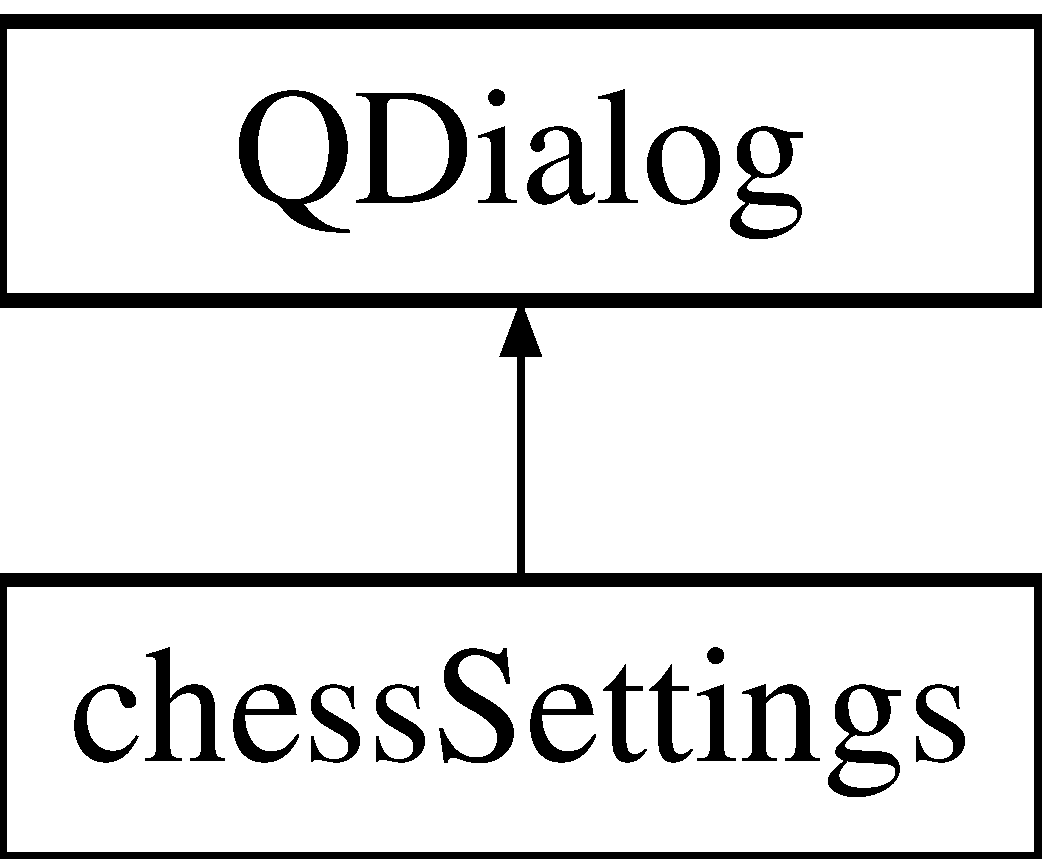
\includegraphics[height=2.000000cm]{classchess_settings}
\end{center}
\end{figure}
\subsection*{Public Member Functions}
\begin{DoxyCompactItemize}
\item 
\mbox{\Hypertarget{classchess_settings_a9b9804678d875a994ec7948c2eff9154}\label{classchess_settings_a9b9804678d875a994ec7948c2eff9154}} 
{\bfseries chess\+Settings} (\hyperlink{classchess_board}{chess\+Board} $\ast$board, Q\+Widget $\ast$parent=0)
\end{DoxyCompactItemize}
\subsection*{Public Attributes}
\begin{DoxyCompactItemize}
\item 
\mbox{\Hypertarget{classchess_settings_a8175026258f6aff812f8c57ad076c00b}\label{classchess_settings_a8175026258f6aff812f8c57ad076c00b}} 
Q\+String {\bfseries temp\+White}
\item 
\mbox{\Hypertarget{classchess_settings_a3ac3ceb3f0488724d5483c1dfadf358a}\label{classchess_settings_a3ac3ceb3f0488724d5483c1dfadf358a}} 
Q\+String {\bfseries temp\+Black}
\item 
\mbox{\Hypertarget{classchess_settings_a1ca15b3fd765819f7227332999a79244}\label{classchess_settings_a1ca15b3fd765819f7227332999a79244}} 
Q\+String {\bfseries temp\+Select}
\item 
\mbox{\Hypertarget{classchess_settings_a0fac91652a3084376ca48fcd37b1100e}\label{classchess_settings_a0fac91652a3084376ca48fcd37b1100e}} 
Q\+String {\bfseries temp\+Attack}
\end{DoxyCompactItemize}


\subsection{Detailed Description}
Odpowiada za prawidłowe wyświetlanie i działanie okna ustawień. 

Tworzy nowe okno ustawień korzystając z klasy bazowej Q\+Dialog. Oferuje zmianę kolorów szachownicy. 

The documentation for this class was generated from the following files\+:\begin{DoxyCompactItemize}
\item 
chesssettings.\+h\item 
chesssettings.\+cpp\end{DoxyCompactItemize}

\hypertarget{classchess_square}{}\section{chess\+Square Class Reference}
\label{classchess_square}\index{chess\+Square@{chess\+Square}}


Klasa reprezentująca pojedyncze pole na szachownicy.  


Inheritance diagram for chess\+Square\+:\begin{figure}[H]
\begin{center}
\leavevmode
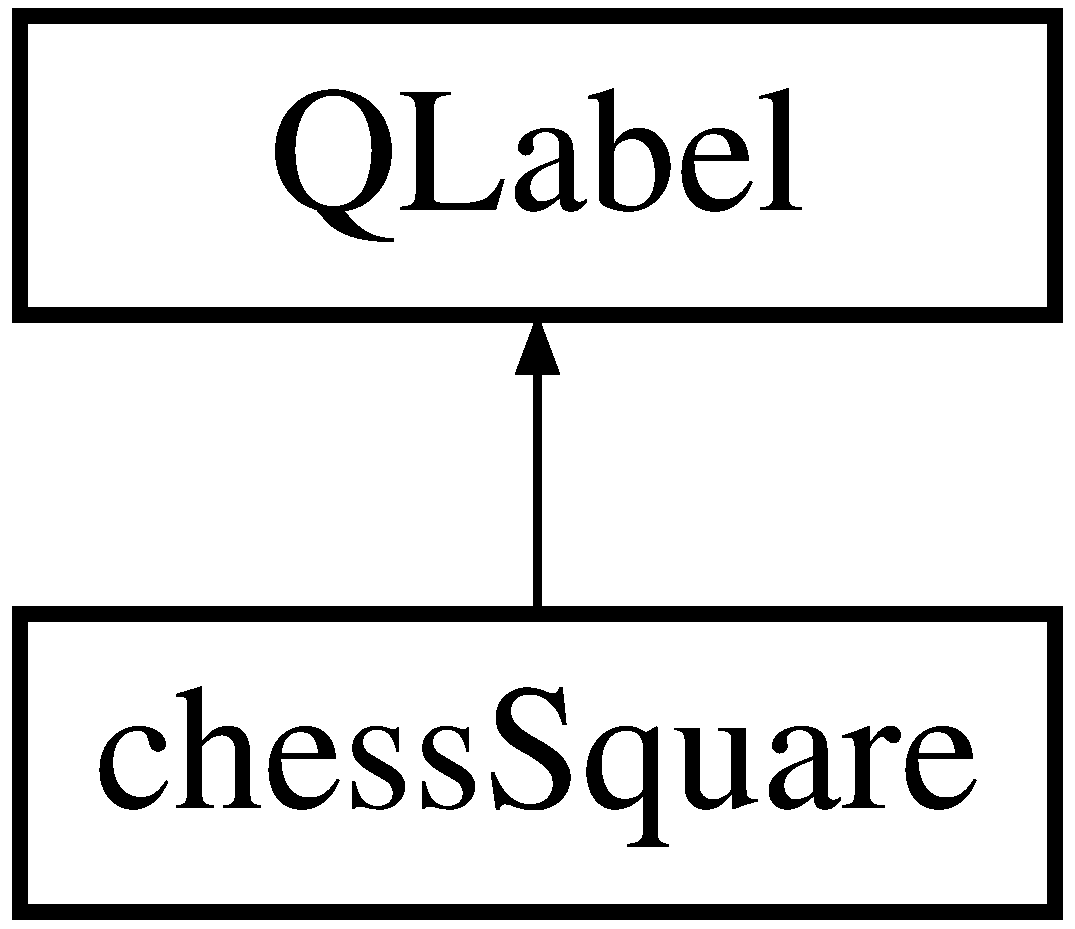
\includegraphics[height=2.000000cm]{classchess_square}
\end{center}
\end{figure}
\subsection*{Signals}
\begin{DoxyCompactItemize}
\item 
\mbox{\Hypertarget{classchess_square_a3d79a4695b0bfa8415da18a7c82819c3}\label{classchess_square_a3d79a4695b0bfa8415da18a7c82819c3}} 
void \hyperlink{classchess_square_a3d79a4695b0bfa8415da18a7c82819c3}{clicked} (int x, int y)
\begin{DoxyCompactList}\small\item\em Sygnał emitowany w przypadku gdy użytkownik kliknął w aktywne pole. \end{DoxyCompactList}\end{DoxyCompactItemize}
\subsection*{Public Member Functions}
\begin{DoxyCompactItemize}
\item 
\mbox{\Hypertarget{classchess_square_a818660e4b5fc11c1749a9af5b9a35aff}\label{classchess_square_a818660e4b5fc11c1749a9af5b9a35aff}} 
{\bfseries chess\+Square} (int col, int row, Q\+Widget $\ast$parent=nullptr)
\item 
\mbox{\Hypertarget{classchess_square_a2393c2aee673f38f121a82562707c740}\label{classchess_square_a2393c2aee673f38f121a82562707c740}} 
void \hyperlink{classchess_square_a2393c2aee673f38f121a82562707c740}{set\+Active} (bool active)
\begin{DoxyCompactList}\small\item\em Ustawia pole jako aktywne (w zależności od wartości active) \end{DoxyCompactList}\item 
\mbox{\Hypertarget{classchess_square_a36cdc0a51aa436eb4fe0ee70cfc80bc9}\label{classchess_square_a36cdc0a51aa436eb4fe0ee70cfc80bc9}} 
void \hyperlink{classchess_square_a36cdc0a51aa436eb4fe0ee70cfc80bc9}{set\+Active} (Q\+String color)
\begin{DoxyCompactList}\small\item\em Ustawia pole jako aktywne i dodatkowo ustawia tymczasowy kolor tła. \end{DoxyCompactList}\item 
\mbox{\Hypertarget{classchess_square_ac8ae6f86143d988ab3c9d54c89c2784f}\label{classchess_square_ac8ae6f86143d988ab3c9d54c89c2784f}} 
bool \hyperlink{classchess_square_ac8ae6f86143d988ab3c9d54c89c2784f}{is\+Piece} ()
\begin{DoxyCompactList}\small\item\em Funkcja sprawdzająca czy na danym polu znajduje się figura. \end{DoxyCompactList}\item 
\mbox{\Hypertarget{classchess_square_ad099713945d1e0a01514cf8b939a34b1}\label{classchess_square_ad099713945d1e0a01514cf8b939a34b1}} 
bool \hyperlink{classchess_square_ad099713945d1e0a01514cf8b939a34b1}{is\+Active} ()
\begin{DoxyCompactList}\small\item\em Zwraca true albo false w zależności czy pole jest aktywne. \end{DoxyCompactList}\item 
\mbox{\Hypertarget{classchess_square_a2fee406370161f95d9a4ff9b0e82c436}\label{classchess_square_a2fee406370161f95d9a4ff9b0e82c436}} 
\hyperlink{classchess_piece}{chess\+Piece} $\ast$ \hyperlink{classchess_square_a2fee406370161f95d9a4ff9b0e82c436}{get\+Piece} ()
\begin{DoxyCompactList}\small\item\em Zwraca figurę z danego pola. \end{DoxyCompactList}\item 
\mbox{\Hypertarget{classchess_square_aa7cbc607deb4a7e4844553e3c74076a1}\label{classchess_square_aa7cbc607deb4a7e4844553e3c74076a1}} 
void \hyperlink{classchess_square_aa7cbc607deb4a7e4844553e3c74076a1}{set\+Piece} (\hyperlink{classchess_piece}{chess\+Piece} $\ast$piece)
\begin{DoxyCompactList}\small\item\em Ustawia figurę na polu. \end{DoxyCompactList}\item 
\mbox{\Hypertarget{classchess_square_ace9bb5543d5e8a2354a979bd7dc95c5c}\label{classchess_square_ace9bb5543d5e8a2354a979bd7dc95c5c}} 
void \hyperlink{classchess_square_ace9bb5543d5e8a2354a979bd7dc95c5c}{remove\+Piece} ()
\begin{DoxyCompactList}\small\item\em Usuwa figurę z pola. \end{DoxyCompactList}\item 
\mbox{\Hypertarget{classchess_square_a2834d87001da98346f34e72168b70ea7}\label{classchess_square_a2834d87001da98346f34e72168b70ea7}} 
void \hyperlink{classchess_square_a2834d87001da98346f34e72168b70ea7}{set\+Background\+Color} (Q\+String color)
\begin{DoxyCompactList}\small\item\em Ustawia nowy domyślny kolor tła. \end{DoxyCompactList}\item 
\mbox{\Hypertarget{classchess_square_a370b3b5cffd0d7fa91ac23f107e062e5}\label{classchess_square_a370b3b5cffd0d7fa91ac23f107e062e5}} 
Q\+String \hyperlink{classchess_square_a370b3b5cffd0d7fa91ac23f107e062e5}{to\+Chess\+Notation} ()
\begin{DoxyCompactList}\small\item\em Zwraca współrzędne zapisane w notacji szachowej. \end{DoxyCompactList}\end{DoxyCompactItemize}
\subsection*{Protected Member Functions}
\begin{DoxyCompactItemize}
\item 
\mbox{\Hypertarget{classchess_square_a237c7ccd0ba13d99c0f6eff2162fbf48}\label{classchess_square_a237c7ccd0ba13d99c0f6eff2162fbf48}} 
void \hyperlink{classchess_square_a237c7ccd0ba13d99c0f6eff2162fbf48}{mouse\+Press\+Event} (Q\+Mouse\+Event $\ast$event)
\begin{DoxyCompactList}\small\item\em Funkcja określająca zachowanie programu w przypadku kliknięcia w pole. \end{DoxyCompactList}\end{DoxyCompactItemize}


\subsection{Detailed Description}
Klasa reprezentująca pojedyncze pole na szachownicy. 

Klasa ta dziedziczy po Q\+Label. Odpowiada za prawidłowe wyświetlanie pojedynczego pola na szachownicy. Każde pole posiada atrybut active, określające czy jest ono aktywne. Tylko aktywne pola mogą być wybierane / zaznaczane przez użytkownika. 

The documentation for this class was generated from the following files\+:\begin{DoxyCompactItemize}
\item 
chesssquare.\+h\item 
chesssquare.\+cpp\end{DoxyCompactItemize}

%--- End generated contents ---

% Index
\backmatter
\newpage
\phantomsection
\clearemptydoublepage
\addcontentsline{toc}{chapter}{Index}
\printindex

\end{document}
